\documentclass[11pt]{article}
\usepackage[margin=1in]{geometry}
\usepackage{amsmath,amssymb,booktabs,graphicx,tabularx,float}
\usepackage[T1]{fontenc}
\usepackage{lmodern}
\usepackage[round]{natbib}
\usepackage[hidelinks]{hyperref}
\newcommand{\Mult}{2.80}
\newcommand{\MultK}{3.42}
\newcommand{\K}{5}
\newcommand{\KWord}{five}
\newcommand{\KOrd}{fifth}
\newcommand{\MultThree}{3.24}
\newcommand{\Tau}{0.66}
\newcommand{\SDIndex}{0.50}
\newcommand{\SDQ}{0.81}
\newcommand{\Rho}{0.24}
\newcommand{\BetaStar}{0.43}
\newcommand{\DQMean}{0.31}
\newcommand{\DQMin}{0.29}
\newcommand{\DQMax}{0.33}
\newcommand{\NStarMain}{126}
\newcommand{\NStarQ}{187}
\newcommand{\NStarQEffective}{479}
\newcommand{\Reps}{2{,}000}
\newcommand{\RepsHet}{1{,}000}
\newcommand{\SimPowMainTwoHundred}{94\%}
\newcommand{\AnaPowMainTwoHundred}{94\%}
\newcommand{\SizeMin}{4.5\%}
\newcommand{\SizeMax}{5.8\%}
\newcommand{\NMin}{30}
\newcommand{\SimPowQAnyTwoHundred}{80\%}
\newcommand{\SimHetHalfEightHundred}{86\%}
\newcommand{\AnaHetHalfEightHundred}{87\%}
\newcommand{\SimHetTwoThreeThousand}{87\%}
\newcommand{\AnaHetTwoThreeThousand}{85\%}
\newcommand{\NDims}{3}
\newcommand{\PUneq}{0.25}
\newcommand{\RepsHetTwo}{1{,}000}
\newcommand{\NStarCellOne}{388}
\newcommand{\NStarCellTwo}{880}
\newcommand{\NStarCellThree}{1{,}637}
\newcommand{\NStarDiffOne}{671}
\newcommand{\NStarDiffTwo}{2{,}681}
\newcommand{\NStarDiffThree}{8{,}038}
\newcommand{\NStarDiffOneUneq}{894}
\newcommand{\NStarDiffTwoUneq}{3{,}574}
\newcommand{\NStarCellOneUneq}{776}
\newcommand{\FamCellOne}{6}
\newcommand{\FamCellTwo}{12}
\newcommand{\FamCellThree}{8}
\newcommand{\FamDiffOne}{3}
\newcommand{\FamDiffTwo}{3}
\newcommand{\FamDiffThree}{1}
\newcommand{\FamQHalf}{30}
\newcommand{\DSum}{0.3}
\newcommand{\DQSum}{0.18}
\newcommand{\SimPowMainTwoHundredLow}{11\%}
\newcommand{\SimPowMainThousandLow}{39\%}
\newcommand{\SimPowMainTwoHundredMid}{54\%}
\newcommand{\SimPowMainThousandMid}{100\%}
\newcommand{\NStarMainLow}{3{,}140}
\newcommand{\NMax}{1{,}000}
\newcommand{\MDEMainFifty}{0.79}
\newcommand{\MDEMainHundred}{0.56}
\newcommand{\MDEMainTwoHundred}{0.40}
\newcommand{\MDEMainFourHundred}{0.28}
\newcommand{\Shrink}{0.62}
\newcommand{\DTarget}{0.50}
\newcommand{\NStarQHalfEff}{1{,}302}
\newcommand{\NStarMainThree}{349}
\newcommand{\BReg}{2{,}000}
\newcommand{\BSim}{199}
\newcommand{\RepsThr}{500}
\newcommand{\NGrid}{5}
\newcommand{\GridLo}{50\%}
\newcommand{\GridHi}{110\%}
\newcommand{\RoundTo}{10}
\newcommand{\RWErr}{3\%}
\newcommand{\BonfSimLo}{95\%}
\newcommand{\BonfSimHi}{103\%}
\newcommand{\RWRatioLo}{70\%}
\newcommand{\RWRatioHi}{83\%}
\newcommand{\NCapped}{3}
\newcommand{\NThr}{19}
\newcommand{\NStarQRW}{150}
\newcommand{\NStarQEffRW}{390}
\newcommand{\NStarQHalfEffRW}{1{,}010}
\newcommand{\NStarQHalfRW}{390}
\newcommand{\NStarQHalf}{509}
\newcommand{\NStarCellOneRW}{320}
\newcommand{\NStarCellTwoRW}{690}
\newcommand{\NStarCellThreeRW}{1{,}290}
\newcommand{\NStarDiffOneRW}{660}
\newcommand{\NStarDiffTwoRW}{2{,}681}
\newcommand{\NStarCellOneUneqRW}{540}
\newcommand{\NStarDiffOneUneqRW}{880}
\newcommand{\SimPowQAvgTwoHundred}{44\%}
\newcommand{\DeltaLow}{0.05}
\newcommand{\StepsLow}{0.25}
\newcommand{\PerHundredLow}{25}
\newcommand{\AllQLow}{5\%}
\newcommand{\FlipLow}{13\%}
\newcommand{\DeltaLowMid}{0.10}
\newcommand{\StepsLowMid}{0.50}
\newcommand{\PerHundredLowMid}{50}
\newcommand{\AllQLowMid}{10\%}
\newcommand{\FlipLowMid}{25\%}
\newcommand{\DeltaMid}{0.15}
\newcommand{\StepsMid}{0.75}
\newcommand{\PerHundredMid}{75}
\newcommand{\AllQMid}{15\%}
\newcommand{\FlipMid}{38\%}
\newcommand{\DeltaMidHigh}{0.20}
\newcommand{\StepsMidHigh}{1.00}
\newcommand{\PerHundredMidHigh}{100}
\newcommand{\AllQMidHigh}{20\%}
\newcommand{\FlipMidHigh}{50\%}
\newcommand{\DeltaHigh}{0.25}
\newcommand{\StepsHigh}{1.25}
\newcommand{\PerHundredHigh}{125}
\newcommand{\AllQHigh}{25\%}
\newcommand{\FlipHigh}{63\%}

\setlength{\parskip}{4pt}
\setlength{\parindent}{0pt}

\title{Power and a staged analysis plan for the Proposition 40 survey experiment}
\author{Fernando Hoces de la Guardia \\ \normalsize Pre-analysis plan, appendix on power}
\date{19 October 2026}

\begin{document}
\maketitle

\textbf{A note on this document.} This appendix, like the pre-analysis plan it belongs to, was
drafted with the assistance of Claude Code. It is unclear whether the survey will draw any
responses at all. The plan was written for the optimistic case, in which enough people respond for
a study to be conducted with the data, so that the analysis is fixed before any response is seen.
\textbf{At this point, it is the opinion of the author that no human should spend much time
reading this pre-analysis plan. It is only intended as a record.}

\section{Why this appendix}

We do not know how many people will answer the survey. It may be a few dozen or a few hundred.
The plan therefore registers one main hypothesis with one outcome, which is tested whatever the
number of responses. It also registers further analyses, each run only if the realized number of
responses is large enough for that analysis to detect an effect of a stated size. This appendix
gives the formulas behind those thresholds, checks them with simulations of the registered
estimator, and states the rule that decides which analyses are run.

The experiment mainly tests the salience of the comparison when respondents choose the input
values. Respondents reach the survey through two entry points. The explorer (forms 3 and 4) is
opened from the comparison explorer, so these respondents have all seen the two estimates. The
share link (forms 5 and 6) brings a mix of respondents who have seen them and respondents who have
not. An earlier design had a third entry point, a landing panel. It has been removed.

Every number below is computed by \texttt{comparison/survey/power/sim.py} and read into this
document from its output. None is typed by hand.

\section{Summary: responses needed to detect 0.3 standard deviations}\label{sec:summary}

Table~\ref{tab:summary} gives the smallest number of responses at which each analysis has 80\%
power against an effect of $\DSum$ standard deviations, at the 5\% level with the Romano-Wolf
adjustment inside each family (Section~\ref{sec:rw}). Expertise and prior exposure are split
50/50. The entry point is split $\PExpl$ explorer and $\PShare$ share link. Column $N^{*}$ is
the Romano-Wolf threshold from the simulations of Section~\ref{sec:rwthr}. Column Bound is the
closed-form Bonferroni bound, which is at or above it. For the \KWord{} questions, column A is an effect of
$\DSum$ standard deviations on one question. Column B is the smaller effect on each question,
about $\DQSum$, that goes with an effect of $\DSum$ on the index (equation~\eqref{eq:shrink}). For
heterogeneity, column A is the effect inside one cell and column B is the highest-order difference
of effects (Section~\ref{sec:het}). Each family covers every combination of the $D = \NDims$
candidate dimensions at that order.

\begin{table}[H]
  \centering
  \small
  \begin{tabularx}{\textwidth}{c X rrr rrr}
\toprule
 & & \multicolumn{3}{c}{A} & \multicolumn{3}{c}{B} \\
\cmidrule(lr){3-5} \cmidrule(lr){6-8}
 & Analysis & Tests $m$ & $N^{*}$ & Bound & Tests $m$ & $N^{*}$ & Bound \\
\midrule
1 & Main hypothesis H1: the lean index & 1 & 349 &  &  &  &  \\
2 & H1 by outcome, each of the five questions. A: 0.3 SD on a question. B: the question-level effect that matches 0.3 SD on the index & 5 & 440 & 520 & 5 & 1,110 & 1,410 \\
3 & Heterogeneity, one dimension at a time (3 combinations). A: the effect inside each of 2 cells. B: the difference between the two halves, in one family with H5 & 6 & 920 & 1,346 & 4 & 1,983$^{\dagger}$ & 1,983 \\
4 & Heterogeneity, two dimensions at a time (3 combinations). A: the effect inside each of 4 cells. B: the 2-way difference & 12 & 2,010 & 3,054 & 3 & 7,090 & 7,445 \\
5 & Heterogeneity, three dimensions at a time (1 combination). A: the effect inside each of 8 cells. B: the 3-way difference & 8 & 3,850 & 5,684 & 1 & 23,256 &  \\
\bottomrule
\end{tabularx}

  \caption{Responses needed for 80\% power against an effect of $\DSum$ standard deviations,
  with the shares of Section~\ref{sec:sim}. $N^{*}$: the simulated Romano-Wolf threshold, rounded up to the next $\RoundTo$.
  Bound: the Bonferroni bound from equations~\eqref{eq:nstar}, \eqref{eq:shrink}
  and~\eqref{eq:nstar-het}. A single test ($m = 1$) needs no adjustment, so its $N^{*}$ comes from
  the formula. $^{\dagger}$The simulation found no Romano-Wolf threshold below the bound, so the
  bound is kept.}
  \label{tab:summary}
\end{table}

\section{Setup}

Respondent $i = 1, \dots, N$ is assigned to treatment, $T_i = 1$, or control, $T_i = 0$, with
probability $1/2$, within two entry-point strata, the explorer and the share link. On each of the $K = \K$ required questions the
answer is coded
\[
  y_{ik} = \begin{cases} +1 & \text{the BSZ value} \\ -1 & \text{the JR value} \\ \phantom{+}0 & \text{about equally credible, or unsure.} \end{cases}
\]
The primary outcome is the lean index, $\mathrm{Lean}_i = \frac{1}{K} \sum_{k=1}^{K} y_{ik}$. The
main hypothesis is tested with
\begin{equation}
  \mathrm{Lean}_i = a + b\,T_i + g\,E_i + e_i,
  \qquad H_1\colon b = 0 \text{ against } b \neq 0, \label{eq:main}
\end{equation}
with the explorer indicator $E_i$ and HC2 standard errors.

Effects are stated in standard-deviation units of the outcome in the control group: a
standardized effect $d = b/\sigma$. This avoids guessing the outcome's spread, which we cannot know
before the data arrive.

\section{Multiple testing}\label{sec:rw}

\paragraph{Families.} The main hypothesis H1 is one test and is not adjusted. Every other analysis
is a family of tests, and each family is adjusted on its own. The families are the \KWord{}
question-level tests, the questions inside each half, the effects inside the cells (one family per
order), the one-dimension differences (H2 to H4, joined by H5), and the two-way differences
(Section~\ref{sec:het}). The three-way difference is a single test.

\paragraph{The procedure.} Each family is adjusted with the Romano-Wolf step-down procedure
\citep{romano2005stepwise}, computed as in \citet*{clarke2020romano}. It works with studentized
statistics, $t_j = \hat b_j / \widehat{\mathrm{se}}_j$, from the registered equations with HC2
standard errors. A pairs bootstrap redraws respondents with replacement within each entry-point
stratum, keeping each stratum's size. Every regression of the family is re-estimated on the same
bootstrap sample. Draw $r$ gives $t^{*}_{j,r} = |\hat b^{*}_{j,r} - \hat b_j| /
\widehat{\mathrm{se}}^{*}_{j,r}$. Centering at the estimate makes the draws mimic the statistics when
every null hypothesis is true. Order the tests so that $|t_{(1)}| \ge \dots \ge |t_{(S)}|$. With $B$
draws, the adjusted p-value of test $(s)$ is
\[
  p_{(s)} = \max_{s' \le s} \; \frac{1 + \#\bigl\{r : \max_{j \ge s'} t^{*}_{(j),r} \ge |t_{(s')}|\bigr\}}{1 + B}.
\]
The first test is compared with the maximum over all tests, the second with the maximum over all
tests but the first, and so on down the list. A test is rejected when its adjusted p-value is at
most 5\%. The registered analysis uses $B = \BReg$ draws.

\paragraph{Why it fits.} The procedure uses the joint distribution of the statistics, so it charges
less for tests that move together. The \KWord{} questions share one latent lean, with an average
correlation of $\Rho$ in the simulated population of Section~\ref{sec:sim}. The cells of different
dimensions share respondents. Bonferroni's method, and Holm's method that an earlier draft of this
appendix used, ignore this correlation and so give up power. When the tests are close to
independent, as the differences across independent dimensions are, Romano-Wolf gains little.

\paragraph{Bounds.} In large samples, the Romano-Wolf critical value at the first step is at most
the Bonferroni critical value $z_{1-\alpha/(2m)}$, and later steps use smaller ones. A threshold
computed with the Bonferroni critical value is therefore an upper bound on the Romano-Wolf
threshold. The formulas below use this bound because it has a closed form. Section~\ref{sec:rwthr}
simulates the Romano-Wolf thresholds themselves.

\section{Analytic minimum detectable effects}

Let $M(m) = z_{1-\alpha/(2m)} + z_{1-\kappa}$ for a two-sided test at level $\alpha = 0.05$ with power
$1-\kappa = 0.80$, where $m$ is the number of tests in the family. The first term is the
Bonferroni critical value, so $M(m)$ gives upper bounds on the Romano-Wolf thresholds
(Section~\ref{sec:rw}). Numerically $M(1) = \Mult$, $M(3) = \MultThree$ and $M(\K) = \MultK$.

\paragraph{Main effect.} With half of $N$ treated,
$\mathrm{Var}(\hat b) = \sigma^2 \left(\frac{1}{N/2} + \frac{1}{N/2}\right) = 4\sigma^2/N$, so
\begin{equation}
  \mathrm{MDE}_{\text{main}}(N, m) = \frac{2\,M(m)}{\sqrt{N}}. \label{eq:mde-main}
\end{equation}
With $N = 50, 100, 200, 400$ responses the main test detects standardized effects of
$\MDEMainFifty$, $\MDEMainHundred$, $\MDEMainTwoHundred$ and $\MDEMainFourHundred$.

\paragraph{Threshold.} Setting the MDE equal to a target $d^{*}$ and solving for $N$ gives the
number of responses the analysis needs:
\begin{equation}
  N^{*}_{\text{main}}(d^{*}, m) = \left(\frac{2M(m)}{d^{*}}\right)^{2}. \label{eq:nstar}
\end{equation}

\section{Heterogeneity by order}\label{sec:het}

\paragraph{The candidate dimensions.} The plan declares $D = \NDims$ binary dimensions, all
recorded before treatment: expertise (Yes or Somewhat, against No), prior exposure (No, against Yes
or Not sure), and entry point (the explorer, against the share link). The entry point is also the
stratum, so for it the stratum indicator already holds the subgroup indicator.
Whether a respondent gives an email is asked on page 1, before treatment, but the plan does not
register it as a dimension. It is descriptive and is not one of the $D$. Any analysis of heterogeneity picks some of the $D$ dimensions, and the more it picks, the
more combinations there are to test and the thinner each cell becomes. The thresholds below count
both.

\paragraph{Cells.} An analysis of order $k$ takes $k$ of the $D$ dimensions. There are
$\binom{D}{k}$ such combinations. Crossing the $k$ dimensions gives $2^k$ cells $c$, with shares
$s_c$ of the sample. The treatment effect inside cell $c$, $\tau_c$, is estimated on $s_c N$
responses, half treated, so
\begin{equation}
  \mathrm{Var}(\hat\tau_c) = \frac{4\sigma^2}{N s_c}. \label{eq:var-cell}
\end{equation}

\paragraph{The $k$-way difference.} The highest-order interaction of a combination is the
alternating sum of the cell effects,
\[
  \Delta_k = \sum_{c} (-1)^{\,k - |c|}\, \tau_c ,
\]
where $|c|$ is the number of the $k$ dimensions at 1 in cell $c$. For $k = 1$ this is
$\tau_1 - \tau_0$, the difference between two subgroups' effects. For $k = 2$ it is
$(\tau_{11} - \tau_{10}) - (\tau_{01} - \tau_{00})$, a difference of differences. In the saturated
regression with 0/1 indicators, $\Delta_k$ is the coefficient on $T_i \times G_{1i} \times \dots
\times G_{ki}$. The cells hold different respondents, so the estimates are independent and
\begin{equation}
  \mathrm{Var}(\hat\Delta_k) = \sum_{c} \frac{4\sigma^2}{N s_c}. \label{eq:var-diff}
\end{equation}
With equal shares, $s_c = 2^{-k}$, the sum has $2^k$ terms of $2^k$ each:
\[
  \mathrm{Var}(\hat\Delta_k) = 4^k \, \frac{4\sigma^2}{N}, \qquad
  \mathrm{MDE}_{\Delta_k} = 2^k \, \frac{2M(m)}{\sqrt{N}}.
\]
Each added dimension doubles the smallest detectable difference, or multiplies the responses
needed by four. If the dimensions are independent with shares $p_j$, the sum factors:
\[
  \sum_c \frac{1}{s_c} = \prod_{j=1}^{k} \frac{1}{p_j(1-p_j)}.
\]
For $k = 1$ this is the familiar $1/\bigl(p(1-p)\bigr)$.

\paragraph{Families.} The tests of one order form one Romano-Wolf family. For the cell effects of order
$k$ the family has $m = \binom{D}{k} 2^k$ tests: every cell of every combination. For the $k$-way
differences it has $m = \binom{D}{k}$ tests. The one-dimension family also holds H5, the effect
among experts without prior exposure (described with the staged rule), so it has one test more. With $D = \NDims$, the cell families have
$\FamCellOne$, $\FamCellTwo$ and $\FamCellThree$ tests for $k = 1, 2, 3$, and the difference
families have $\FamDiffOne$, $\FamDiffTwo$ and $\FamDiffThree$.

\paragraph{Thresholds.} Setting each MDE equal to $d^{*}$ gives
\begin{equation}
  N^{*}_{\text{cell}}(k) = \frac{1}{\min_c s_c}\left(\frac{2M(m)}{d^{*}}\right)^{2}, \qquad
  N^{*}_{\Delta}(k) = \Bigl(\sum_{c} \frac{1}{s_c}\Bigr)\left(\frac{2M(m)}{d^{*}}\right)^{2},
  \label{eq:nstar-het}
\end{equation}
each with its own family's $m$. Table~\ref{tab:orders} gives them for $k = 1, 2, 3$. By these
bounds, with expertise and exposure split 50/50 and the entry point $\PExpl$ explorer, a
one-dimension difference needs $\NStarDiffOne$ responses, a two-way difference
$\NStarDiffTwo$, and the three-way difference $\NStarDiffThree$. The three-way family is a single test, so its
multiplier is the smallest, and the factor of four per dimension still dominates. The unequal
columns split expertise $\PUneq$ to the rest, independently of the other two. The bound for a cell
family is set by its smallest cell. Every family has cells in the share stratum, so these bounds
are above those for a 50/50 entry point.

\begin{table}[!htbp]
  \centering
  \footnotesize
  \setlength{\tabcolsep}{4pt}
  \begin{tabular}{ccc rrrrr rrrrr}
\toprule
 & & & \multicolumn{5}{c}{Effect inside one cell} & \multicolumn{5}{c}{$k$-way difference of effects} \\
\cmidrule(lr){4-8} \cmidrule(lr){9-13}
$k$ & $\binom{D}{k}$ & Cells & $m$ & $M$ & 0.5 & 0.3 & 0.5, unequal & $m$ & $M$ & 0.5 & 0.3 & 0.5, unequal \\
\midrule
1 & 3 & 2 & 6 & 3.48 & 485 & 1,346 & 776 & 4 & 3.34 & 714 & 1,983 & 952 \\
2 & 3 & 4 & 12 & 3.71 & 1,100 & 3,054 & 2,199 & 3 & 3.24 & 2,681 & 7,445 & 3,574 \\
3 & 1 & 8 & 8 & 3.58 & 2,047 & 5,684 & 4,093 & 1 & 2.80 & 8,373 & 23,256 & 11,163 \\
\bottomrule
\end{tabular}

  \caption{Responses needed, $N^{*}$, for heterogeneity analyses of order $k$ with $D = \NDims$
  candidate dimensions, from equation~\eqref{eq:nstar-het}. $m$ is the number of tests in the
  order's family and $M = M(m)$, with the Bonferroni critical value, so the entries are upper
  bounds. Table~\ref{tab:n} gives the Romano-Wolf thresholds. Columns 0.5 and 0.3 give $d^{*}$
  with expertise and exposure split 50/50 and the entry point $\PExpl$ explorer. The unequal columns
  use $d^{*} = 0.5$ with expertise split $\PUneq$ to the rest.}
  \label{tab:orders}
\end{table}

The standard deviation $\sigma$ is that of the whole control group. If a dimension explains part
of the spread of the index, the spread inside a cell is smaller and these thresholds are
conservative.

\section{The index and its questions}

The thresholds in~\eqref{eq:nstar} are in standardized units of each analysis's own outcome. An
index and a single question have different spreads, so the same change in answers is a larger
standardized effect on the index than on a question. If treatment moves every question by the same
raw amount $\delta$, each question has standard deviation $\sigma_q$, and the questions are
correlated with average correlation $\rho$, then the index has standard deviation
$\sigma_q\sqrt{\rho + (1-\rho)/K}$ and
\begin{equation}
  d_{\text{question}} = d_{\text{index}} \times \sqrt{\rho + \frac{1-\rho}{K}}. \label{eq:shrink}
\end{equation}
In the simulated population of Section~\ref{sec:sim}, $\rho = \Rho$ and the factor is $\Shrink$. An
effect of $\DTarget$ on the index is an effect of about $\DQMean$ on each question (between $\DQMin$
and $\DQMax$). Detecting that on one question, with Romano-Wolf over \KWord{}, takes about
$\NStarQEffRW$ responses in the simulations (the Bonferroni bound is $\NStarQEffective$). An effect
of $\DTarget$ on each question needs only $\NStarQRW$ (bound $\NStarQ$). This is why the index is the primary outcome: it is the analysis with power at small
samples.

\section{What the effect sizes mean on the index}\label{sec:mag}

A standardized effect is the change in the mean lean index divided by the index's standard
deviation in the control group. The simulated population of Section~\ref{sec:sim} has an index
standard deviation of $\SDIndex$. This spread is an assumption, not a measurement. With it, an
effect of $d$ standard deviations is a change of $d \times \SDIndex$ in the mean index.

The index counts steps. An answer moves one step when it goes from neutral to a study's value, or
from the other study's value to neutral. One step on one answer moves that respondent's index by
$1/K$, one \KOrd{}. A switch from one study's value to the other's is two steps, or two \KOrd{}s. The
same change in the mean index can therefore come about in several ways. Table~\ref{tab:mag} gives
three for each of five effect sizes, from 0.1 to 0.5. All are counted against the control group,
with every move toward the same study's value.

\begin{itemize}
  \item \textbf{0.1 standard deviations} is a change of $\DeltaLow$ in the mean index. For every 100
  treated respondents, that is $\PerHundredLow$ one-step moves in all, or $\StepsLow$ of a step per
  respondent. It is also what results if $\AllQLow$ of treated respondents move all \KWord{} answers
  one step, or if $\FlipLow$ switch one answer from one study's value to the other's.
  \item \textbf{0.3 standard deviations} is a change of $\DeltaMid$. That is $\PerHundredMid$ one-step
  moves per 100 treated respondents, or $\StepsMid$ of a step each. It is also $\AllQMid$ of
  respondents moving all \KWord{} answers one step, or $\FlipMid$ switching one answer from one study's
  value to the other's.
  \item \textbf{0.5 standard deviations} is a change of $\DeltaHigh$. That is $\PerHundredHigh$ one-step
  moves per 100 treated respondents, more than one step each ($\StepsHigh$). It is also
  $\AllQHigh$ of respondents moving all \KWord{} answers one step, or $\FlipHigh$ switching one
  answer from one study's value to the other's.
\end{itemize}

\begin{table}[!htbp]
  \centering
  \small
  \begin{tabular}{c c c c c r}
\toprule
Effect & Index & One-step moves per & Share moving all & Share switching one & Responses for \\
(SD) & points & 100 treated & five answers & answer to the & 80\% power \\
 & & respondents & one step & other value & on H1 \\
\midrule
0.1 & 0.05 & 25 & 5\% & 13\% & 3,140 \\
0.2 & 0.10 & 50 & 10\% & 25\% & 785 \\
0.3 & 0.15 & 75 & 15\% & 38\% & 349 \\
0.4 & 0.20 & 100 & 20\% & 50\% & 197 \\
0.5 & 0.25 & 125 & 25\% & 63\% & 126 \\
\bottomrule
\end{tabular}

  \caption{Five standardized effects in the lean index's own units, with the simulated index
  standard deviation of $\SDIndex$. A one-step move takes one answer from neutral to a study's
  value, or from the other study's value to neutral. The last column is
  $N^{*}_{\text{main}}$ from~\eqref{eq:nstar}.}
  \label{tab:mag}
\end{table}

\section{Simulations}\label{sec:sim}

\paragraph{Data-generating process.} Respondent $i$ has a latent lean $\theta_i \sim
\mathcal{N}(0, \tau^2)$. The latent answer to question $k$ is $\theta_i + a_k + \beta T_i +
\varepsilon_{ik}$ with $\varepsilon_{ik} \sim \mathcal{N}(0, 1)$, and is coded $+1$ above $0.5$,
$-1$ below $-0.5$, and $0$ between. $K$ fixed question intercepts $a_k$ make some questions lean
one way and some the other. $\tau = \Tau$ is calibrated so that the lean index has standard
deviation $\SDIndex$. This spread is an assumption, since no answers exist yet. A single question then has standard
deviation $\SDQ$. For each panel of Figure~\ref{fig:main}, the treatment shift $\beta$ is chosen so
the standardized effect on the index is 0.1, 0.3 or 0.5. For $\DTarget$ it is $\beta = \BetaStar$. Every sample also draws the $D = \NDims$ binary
dimensions, independent of each other. Expertise and prior exposure are each split 50/50 unless
stated. The third dimension is the entry point, which is also the stratum. Of the respondents,
$\PExpl$ enter through the explorer and $\PShare$ through the share link. This split is an
assumption. The
estimator is the registered one: equation~\eqref{eq:main}, with HC2 standard errors and $t$
critical values for a single test. Each point is $\Reps$ replications ($\RepsHet$ for the
heterogeneity curves).

\paragraph{Romano-Wolf inside the simulations.} Each simulated sample runs the whole procedure of
Section~\ref{sec:rw}: the family's regressions, $\BSim$ bootstrap draws within strata, and the
step-down. The simulations use fewer draws than the registered $\BReg$ to save time. Fewer draws
cost a little power, so the simulated thresholds lean high.

For the heterogeneity curves, the latent treatment shift differs across the halves of one
dimension, or across the cells of one pair, so that the standardized $k$-way difference is
$\DTarget$. The other dimensions or pairs of the family carry no difference. For $k = 2$ the shift
is $\pm h/4$ across the four cells of two independent 50/50 dimensions, and the test is on the
coefficient of $T_i \times G_{1i} \times G_{2i}$ in the saturated version of
equation~\eqref{eq:main}. Each replication applies Romano-Wolf to its order's whole family. That
is the $\FamDiffOne$ tests of H2 to H5, or the $\FamDiffTwo$ two-way differences.

\paragraph{Results.} Figure~\ref{fig:main} shows the power of the main test and of a single-question
test, in three panels, one for each true effect on the index. The simulated points lie on the
analytic curves: at $N = 200$ and an effect of $\DTarget$, the main test's simulated power is
$\SimPowMainTwoHundred$ against $\AnaPowMainTwoHundred$ from~\eqref{eq:mde-main}. At 0.3 standard
deviations the main test's power is $\SimPowMainTwoHundredMid$ at $N = 200$ and
$\SimPowMainThousandMid$ at $N = \NMax$. At 0.1 standard deviations it is $\SimPowMainTwoHundredLow$
at $N = 200$ and $\SimPowMainThousandLow$ at $N = \NMax$. Reaching 80\% at that size takes
$\NStarMainLow$ responses. The single
question lags far behind, as~\eqref{eq:shrink} predicts. Its simulated points, with Romano-Wolf over
the \KWord{} questions, lie above the Bonferroni curve, because the questions are correlated. The
probability that at least one of the
\KWord{} questions rejects at $N = 200$ is $\SimPowQAnyTwoHundred$. Under no effect, the main test
rejects in between $\SizeMin$ and $\SizeMax$ of replications for every $N$ from $\NMin$ up, so the
test keeps its 5\% level even with few responses.

\begin{figure}[!htbp]
  \centering
  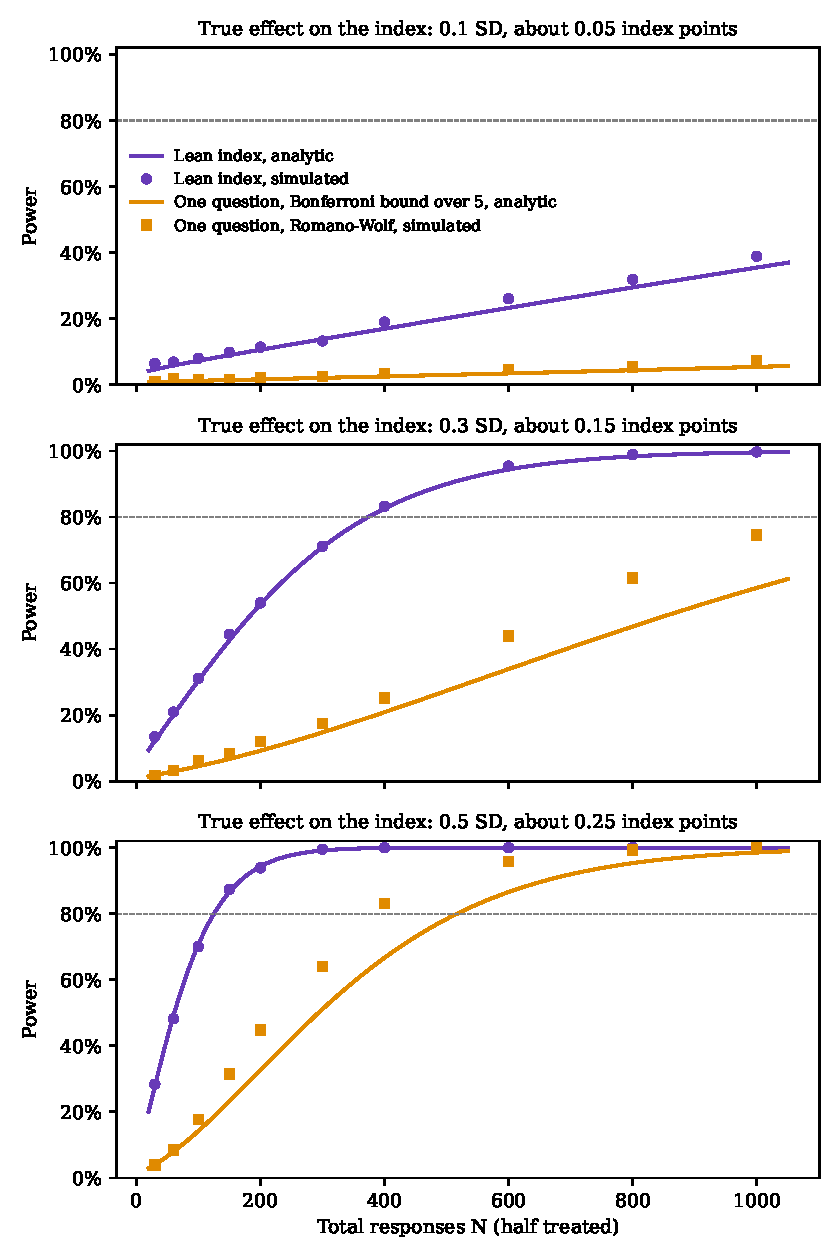
\includegraphics[width=0.85\textwidth]{out/power_main.pdf}
  \caption{Power against total responses for a treatment that shifts the lean index by 0.1, 0.3
  or 0.5 standard deviations (top to bottom). Table~\ref{tab:mag} gives each in index points. Lines:
  equation~\eqref{eq:mde-main}, with the Bonferroni bound for the single question. Points:
  simulations of the registered estimator, with Romano-Wolf over the \KWord{} questions. The dashed
  line is 80\% power.}
  \label{fig:main}
\end{figure}

Figure~\ref{fig:het} does the same for heterogeneity, at a $k$-way difference of $\DTarget$
standard deviations. The simulated Romano-Wolf points lie on the Bonferroni curves. The
differences across independent dimensions are nearly independent tests, and only one carries an
effect, so the step-down gains little here. For one dimension split 50/50, at $N = 800$, the
simulated power is $\SimHetHalfEightHundred$ against $\AnaHetHalfEightHundred$
from~\eqref{eq:nstar-het}. For two dimensions, at $N = 3{,}000$, it is
$\SimHetTwoThreeThousand$ against $\AnaHetTwoThreeThousand$.

\begin{figure}[!htbp]
  \centering
  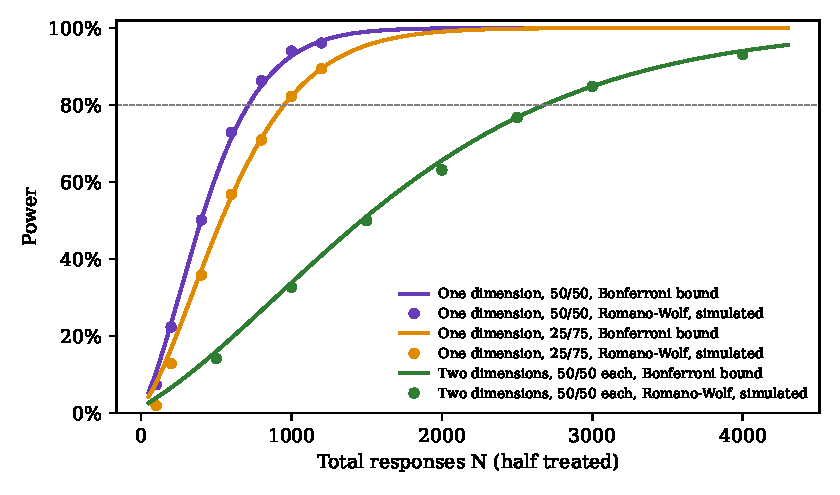
\includegraphics[width=0.9\textwidth]{out/power_het.pdf}
  \caption{Power to detect a $k$-way difference of $\DTarget$ standard deviations: one dimension
  split 50/50 or 25/75 (Romano-Wolf over the $\FamDiffOne$ tests of H2 to H5), and two dimensions split 50/50 each
  (Romano-Wolf over $\FamDiffTwo$). Lines: the Bonferroni bound from equation~\eqref{eq:var-diff}.
  Points: simulations of the registered estimator with the Romano-Wolf step-down.}
  \label{fig:het}
\end{figure}

\subsection{Romano-Wolf thresholds}\label{sec:rwthr}

For each family and target $d^{*}$, the simulation measures power at \NGrid{} values of $N$, from
$\GridLo$ to $\GridHi$ of the Bonferroni bound, with $\RepsThr$ replications each. Power is the share
of replications in which a test with the effect is rejected, averaged over the tests with the
effect. A weighted straight line through $\Phi^{-1}(\text{power})$ against $\sqrt{N}$, the shape of
the normal power curve, gives the $N$ with 80\% power. That $N$, rounded up to the next $\RoundTo$,
is the Romano-Wolf threshold $N^{*}$ of Tables~\ref{tab:summary} and~\ref{tab:n}. Its simulation
standard error is at most $\RWErr$ of its value.

The effect patterns follow what each analysis looks for. For the questions and the cells, treatment
shifts every respondent's latent lean by the same amount, so every test in the family has the
effect: $d^{*}$ on each question, or $d^{*}$ on the index inside each cell. For the differences, one
dimension or one pair carries a difference of $d^{*}$, and the others carry none.

For the questions and the cells, the Romano-Wolf thresholds are $\RWRatioLo$ to $\RWRatioHi$ of the
Bonferroni bounds. For the differences, the tests are nearly independent and only one has an
effect, so Romano-Wolf can gain little. With only $\BSim$ draws, the simulation finds no threshold
below the bound in $\NCapped$ of the $\NThr$ cases, and the tables keep the bound there. Where it
finds one for a difference, the gain is within simulation error. The same
samples, judged against the Bonferroni critical value, reach 80\% power at $\BonfSimLo$ to
$\BonfSimHi$ of the bound. This checks the formulas.

\section{The staged rule}

\paragraph{Rule.} At the close of collection, compute the realized number of responses $N$ and the
realized share $\hat p$ of each pre-treatment subgroup. Run every registered analysis whose
threshold $N^{*}$, evaluated at the realized shares and at the target $d^{*} = \DTarget$, is at
most $N$. For a family of tests, $N^{*}$ is the Romano-Wolf threshold simulated as in
Section~\ref{sec:rwthr}. For a single test, it comes from~\eqref{eq:nstar}
or~\eqref{eq:nstar-het}. Report every other registered analysis as ``not run: below its
threshold'', with the threshold. The main hypothesis is always run and always reported, with its MDE
at the realized $N$. The rule uses only $N$ and pre-treatment shares, which carry no information
about treatment effects, so applying it does not depend on the results.

\paragraph{Heterogeneity by order.} Heterogeneity is unlocked one order at a time. Analyses of one
dimension come first. Analyses of order $k$ are run only if those of order $k - 1$ of the same
kind are run, and only if $N$ reaches their own threshold. With the assumed shares the thresholds already
rise with $k$, so this condition matters only when realized shares are very uneven.

\paragraph{The target.} $d^{*} = \DTarget$ is a medium standardized effect. A smaller target, such as
$0.3$, would make every threshold about $(0.5/0.3)^2 \approx 2.8$ times larger. Table~\ref{tab:n}
gives both.

\begin{table}[!htbp]
  \centering
  \small
  \begin{tabularx}{\textwidth}{l X c rr rr}
\toprule
 & & & \multicolumn{2}{c}{$d^{*} = 0.5$} & \multicolumn{2}{c}{$d^{*} = 0.3$} \\
\cmidrule(lr){4-5} \cmidrule(lr){6-7}
Tier & Analysis & Tests $m$ & $N^{*}$ & Bound & $N^{*}$ & Bound \\
\midrule
0 & H1: lean index, full sample & 1 & 126 &  & 349 &  \\
1 & Each of the five questions & 5 & 150 & 187 & 410 & 520 \\
2a & Effect inside each cell, one dimension at a time (3 combinations, 2 cells each) & 6 & 320 & 388 & 890 & 1,077 \\
2b & Difference between the two halves, one dimension at a time (H2 to H4) & 3 & 660 & 671 & 1,862$^{\dagger}$ & 1,862 \\
3a & Effect inside each cell, two dimensions at a time (3 combinations, 4 cells each) & 12 & 690 & 880 & 1,960 & 2,443 \\
3b & 2-way difference of effects, two dimensions at a time & 3 & 2,681$^{\dagger}$ & 2,681 & 7,445$^{\dagger}$ & 7,445 \\
4a & Effect inside each cell, three dimensions at a time (1 combination, 8 cells each) & 8 & 1,290 & 1,637 & 3,670 & 4,547 \\
4b & 3-way difference of effects, three dimensions at a time (one test) & 1 & 8,038 &  & 22,326 &  \\
5 & Each question inside each half, one dimension at a time & 30 & 390 & 509 & 1,060 & 1,413 \\
\bottomrule
\end{tabularx}

  \caption{Responses needed before each analysis is run. $N^{*}$: the simulated Romano-Wolf
  threshold, rounded up to the next $\RoundTo$. For a single test ($m = 1$), the formula. Bound: the
  Bonferroni bound from equations~\eqref{eq:nstar} and~\eqref{eq:nstar-het}. $^{\dagger}$The
  simulation found no Romano-Wolf threshold below the bound, so the bound is kept. Heterogeneity
  rows assume the shares of Section~\ref{sec:sim}. Row 2b assumes that the H5 subgroup holds a
  quarter of the responses. If it holds half, H5 alone needs $\NStarHFiveHalfRW$. At the close all rows are recomputed at the realized shares.}
  \label{tab:n}
\end{table}

\paragraph{What the tiers mean in practice.} The numbers are the thresholds $N^{*}$ of
Table~\ref{tab:n} at $d^{*} = \DTarget$.
\begin{itemize}
  \item Below $\NStarMain$ responses, only the main test is run. It can detect only effects larger
  than half a standard deviation, and the write-up says so.
  \item From $\NStarQRW$ responses, the \KWord{} questions are each reported (tier 1). By
  equation~\eqref{eq:shrink}, a question-level effect that matches an index effect of $\DTarget$
  needs about $\NStarQEffRW$ responses, so question-level results between the two are reported
  as estimates with confidence intervals, not as tests of a common effect.
  \item From $\NStarCellOneRW$ responses, the effect inside each half of each dimension is reported
  (tier 2a, Romano-Wolf over $\FamCellOne$): experts and non-experts, respondents with and without prior
  exposure, and the explorer against the share link. If one half of expertise holds only a quarter
  of the responses, this needs $\NStarCellOneUneqRW$. The same split by whether a respondent gives an
  email is descriptive only (see below).
  \item From $\NStarDiffOneRW$ responses, the tests that two halves' effects differ are run, together
  with H5 (tier 2b, the plan's H2 to H5, Romano-Wolf over $\FamDiffOne$). With one half holding a
  quarter, the differences need $\NStarDiffOneUneqRW$.
  \item Two dimensions at a time: the effect inside each of the four cells from $\NStarCellTwoRW$
  (tier 3a), and the two-way differences from $\NStarDiffTwoRW$ (tier 3b).
  \item Three dimensions at a time: the effect inside each of the eight cells from
  $\NStarCellThreeRW$ (tier 4a), and the three-way difference, a single test, from
  $\NStarDiffThree$ (tier 4b).
  \item Question-by-subgroup effects, one dimension at a time (tier 5, Romano-Wolf over
  $\FamQHalf$), are reported from $\NStarQHalfRW$ responses. A question-level effect that matches
  an index effect of $\DTarget$ needs about $\NStarQHalfEffRW$ responses once
  equation~\eqref{eq:shrink} is taken into account, so results between the two are read as in
  tier 1, as estimates with confidence intervals.
\end{itemize}

\paragraph{Experts without prior exposure (H5).} H5 is the treatment effect on the lean index
among respondents who answer ``Yes'' or ``Somewhat'' to the expertise question and ``No'' to the
prior-exposure question. Both questions come before treatment. H5 is equation~\eqref{eq:main}
estimated inside this subgroup, with HC2 standard errors. It joins the family of H2 to H4, so
tier 2b has $\FamDiffOne$ tests under one Romano-Wolf adjustment. The tier's threshold is the
larger of two simulated thresholds. In one, the halves of one dimension differ by $\DTarget$
standard deviations. In the other, treatment has an effect of $\DTarget$ on everyone, which H5
must detect inside its subgroup. The simulations draw expertise and exposure 50/50 and
independently, so the subgroup holds a quarter of the responses. The tier then needs
$\NStarDiffOneRW$ responses (bound $\NStarDiffOne$). If the subgroup holds half, H5 alone needs
$\NStarHFiveHalfRW$ (bound $\NStarHFiveHalf$), and H2 to H4 set the tier's threshold. Without
any adjustment, H5 as a single test would need $\NStarHFiveUnadj$ responses at a quarter and
$\NStarHFiveHalfUnadj$ at a half.

\paragraph{Email.} Whether a respondent gives an email is asked on page 1, before treatment (moved
there on 2026-10-18), so treatment cannot change it. The plan does not register it as a dimension,
so analyses split by email are descriptive. They are reported together with the share who give an
email, by arm.

\paragraph{Other dimensions.} A dimension added later raises $D$, which enlarges every family
and every threshold above. It must be registered before the data are seen, and
equation~\eqref{eq:nstar-het} and the simulations are then recomputed with the new $D$. A split on a question asked
after treatment is descriptive only.

\begin{figure}[!htbp]
  \centering
  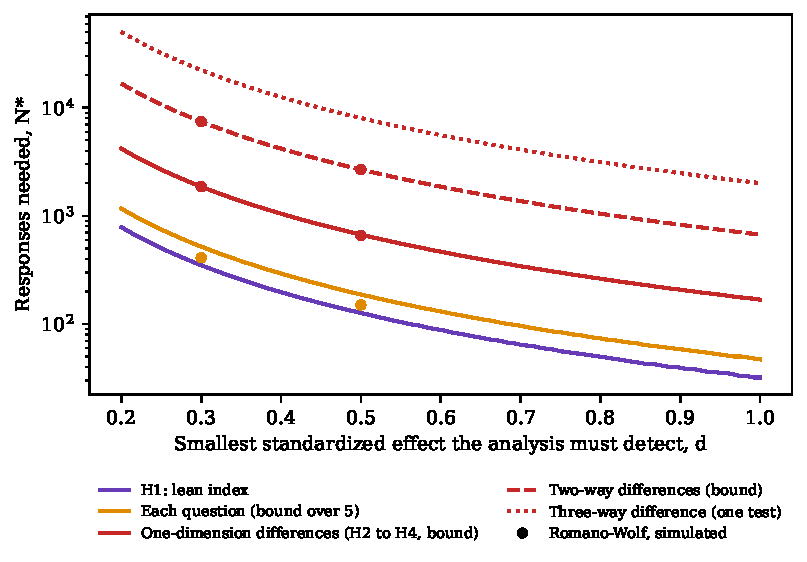
\includegraphics[width=0.9\textwidth]{out/nstar.pdf}
  \caption{Responses needed, $N^{*}$, against the effect the analysis must detect, with the shares
  of Section~\ref{sec:sim}. Lines: equations~\eqref{eq:nstar} and~\eqref{eq:nstar-het}, Bonferroni bounds for the
  families. Points: the simulated Romano-Wolf thresholds at $d = 0.3$ and $\DTarget$. Log scale.}
  \label{fig:nstar}
\end{figure}

\section{Limits}

The thresholds assume equal arms, independent responses, and standardized effects. Unequal arms
raise them slightly. The simulated population is one plausible shape of answers, chosen to match
the assumed spread of the index. If answers are more correlated across questions, the gap between
the index and single questions narrows. If they are less correlated, it widens. None of this
affects the validity of the main test, whose level the simulations confirm at every sample size.
It affects only how large the effects must be to be seen. The Romano-Wolf thresholds also depend on
the assumed effect patterns and correlations. The Bonferroni bounds do not.

The simulations draw the three dimensions independently. Respondents who enter through the
explorer have all seen the two estimates, so many of them may answer ``Yes'' to the prior-exposure
question. Then the cells that cross exposure with the entry point are thin, and their thresholds
rise. The staged rule recomputes every threshold at the realized shares, so it accounts for this
at the close.

\begin{thebibliography}{2}
\bibitem[Clarke et~al.(2020)Clarke, Romano, and Wolf]{clarke2020romano}
Clarke, D., J.~P. Romano, and M.~Wolf (2020). The Romano--Wolf multiple-hypothesis correction in
Stata. \emph{Stata Journal} 20(4), 812--843.

\bibitem[Romano and Wolf(2005)]{romano2005stepwise}
Romano, J.~P. and M.~Wolf (2005). Stepwise multiple testing as formalized data snooping.
\emph{Econometrica} 73(4), 1237--1282.
\end{thebibliography}

\end{document}
